%!TEX root = ../../thesis.tex

The entire LHC Run~I dataset was analysed, corresponding to an integrated luminosity of 
\unit{4.5}{\invfb} at \unit{$\sqrt{s} = 7$}{\TeV} and \unit{20.3}{\invfb} at 
\unit{$\sqrt{s} = 8$}{\TeV}. The major differences of the \unit{7}{\TeV} analysis, with 
respect to \Chapter~\ref{chap:selection}, are the absence of the \twojet bin and the 
dilepton triggers, and the use of a dijet fake factor in the \Wjets background estimation. 
Additionally, the number of \mt bins used in the fit is reduced by a factor of two.
Some minor differences also exist in the object and event selection criteria due to the less 
harsh pile-up environment at \unit{7}{\TeV} (see \Section~\ref{sec:dataset:dataset}).



\subsection{Exclusion, discovery and measurement of \ggHWW}
\label{sec:results:ggF_limits}

The event selection criteria of the \ggHWW analysis are chosen such that the dominant 
production mode of the selected Higgs boson events is ggF. Nevertheless, other production 
modes contribute to the signal acceptance. This effect is small in the 0-jet and 1-jet bins, 
but VBF (\VH) contributes 15\% (10\%) of signal events to the \twojet bin. Such events are 
treated as signal in the fit, and their expected yield is scaled by the same $\mu$ as ggF. 
This has a small effect upon the results, and splitting $\mu$ according to production 
mode shall be revisited in \Section~\ref{sec:results:combined_limits}.

\begin{figure}[p]
	\begin{subfigure}[b]{0.495\textwidth}
		\centering
		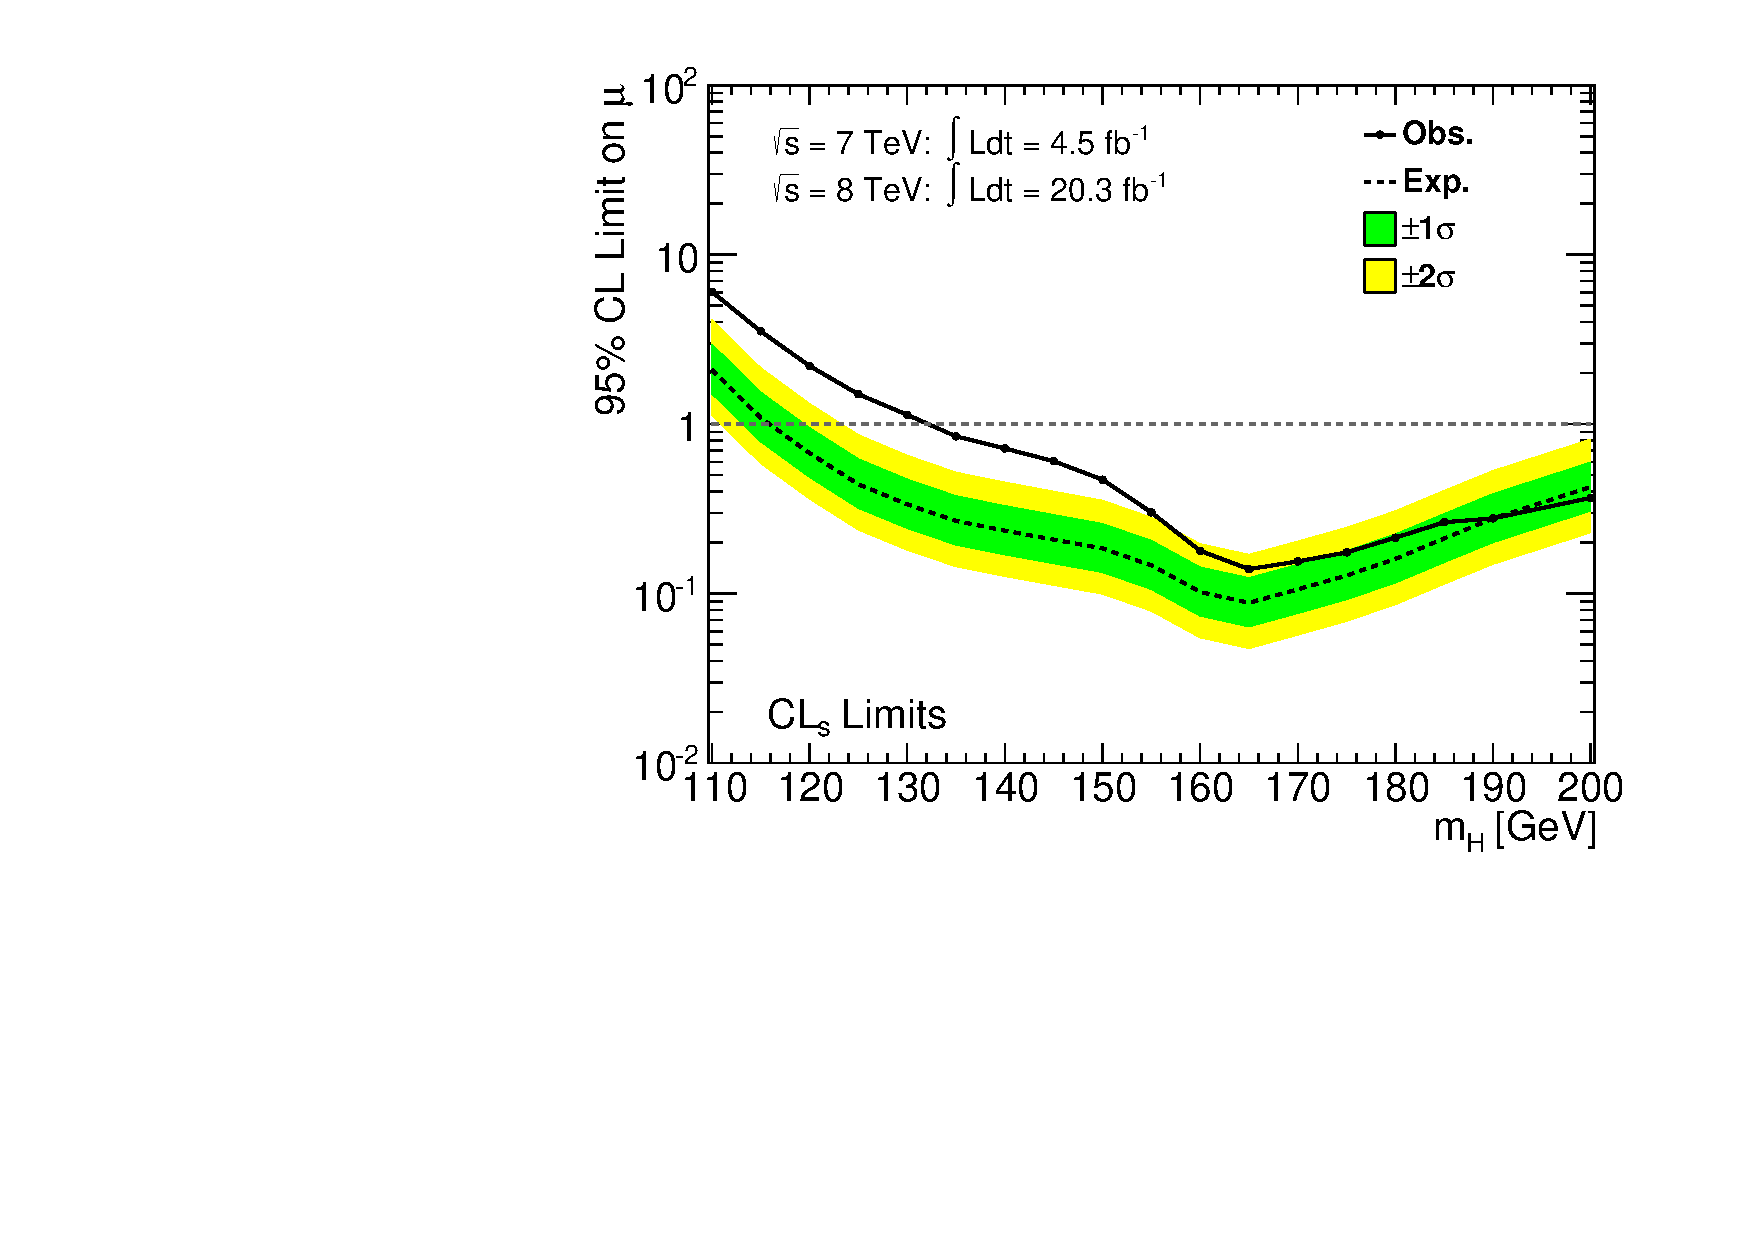
\includegraphics[width=\textwidth,clip=true,trim=0.6cm 0.8cm 1.0cm 0.4cm]{custom_images/limits/cls_ggf_only}
		\caption{Exclusion}
		\label{fig:ggf_results:CLs}
	\end{subfigure}
	\hfill
	\begin{subfigure}[b]{0.495\textwidth}
		\centering
		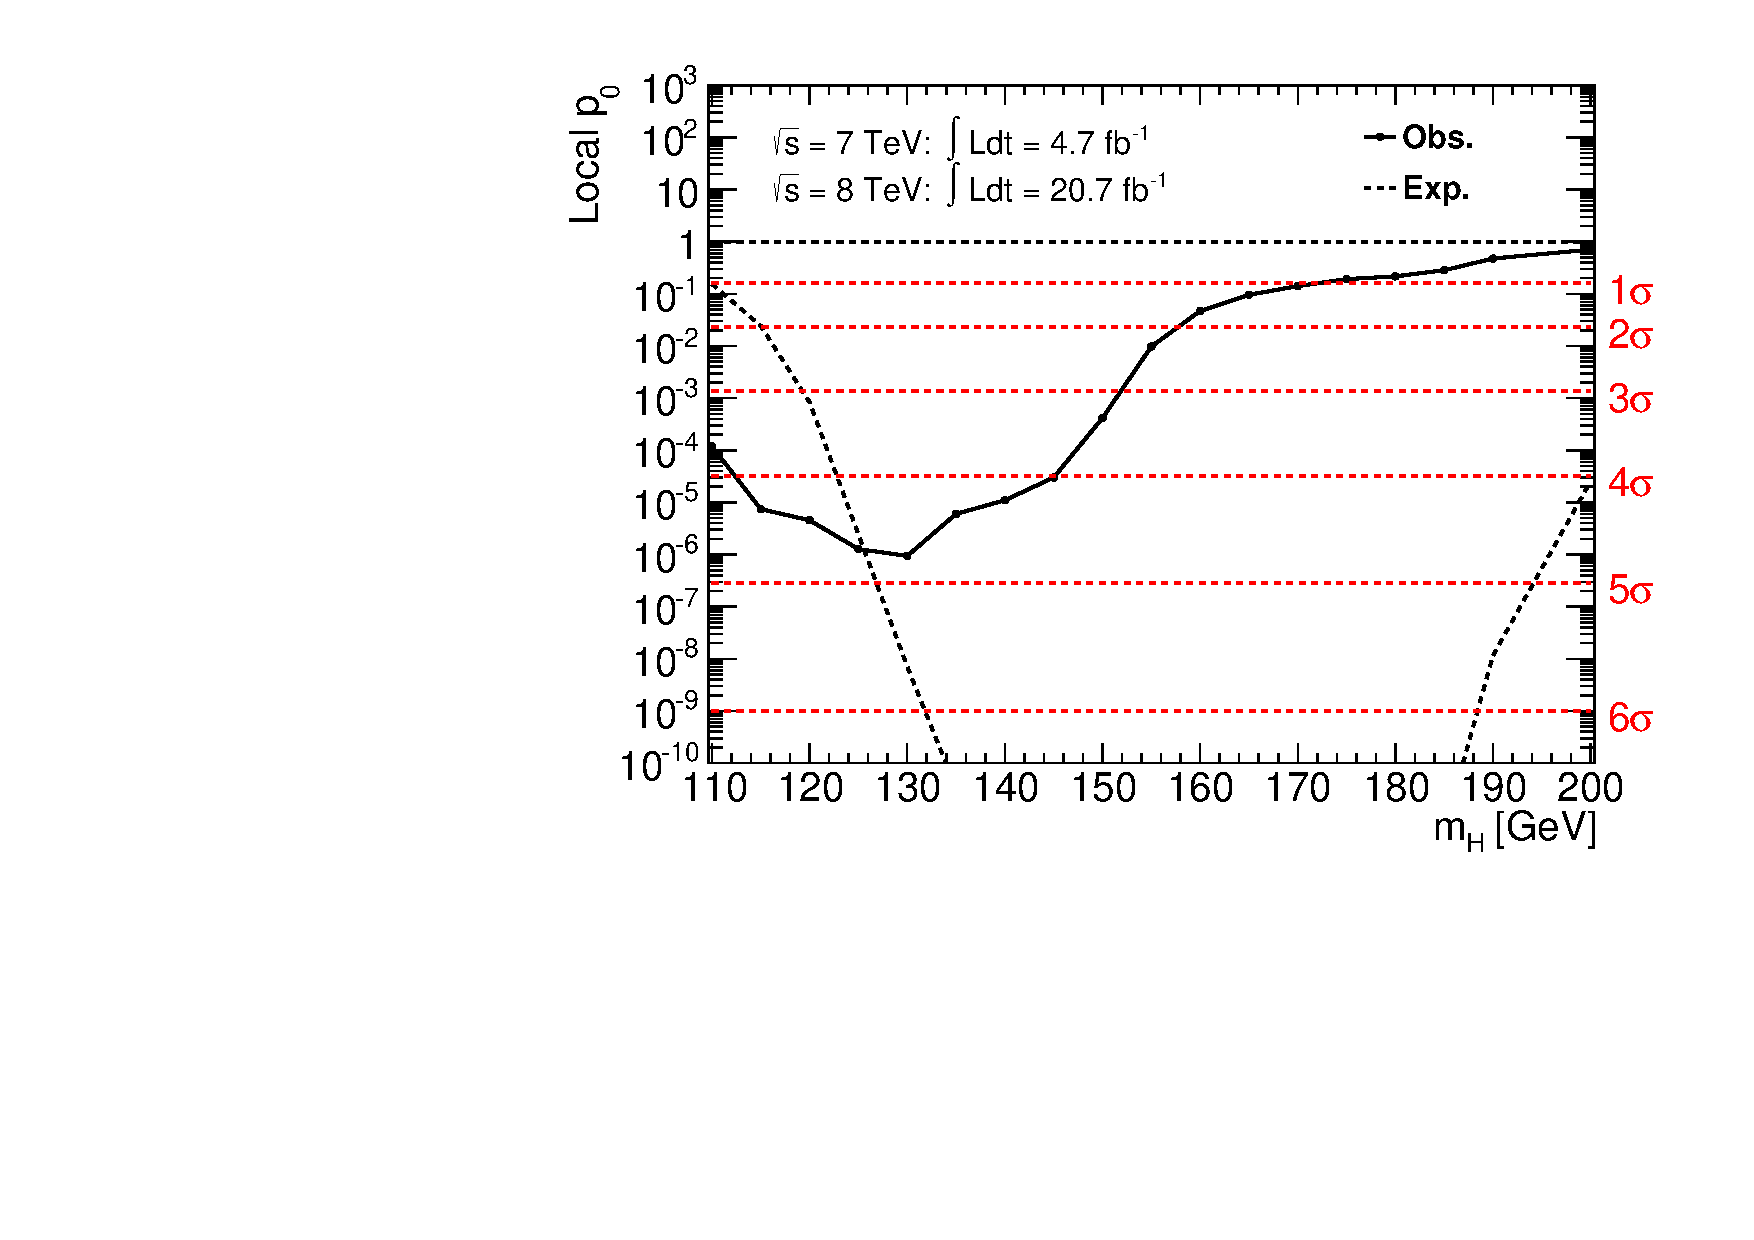
\includegraphics[width=\textwidth,clip=true,trim=0.6cm 0.8cm 1.0cm 0.4cm]{custom_images/limits/p0_ggf_only}
		\caption{Discovery}
		\label{fig:ggf_results:p0}
	\end{subfigure}
	\\[12pt]
	\begin{subfigure}[b]{0.495\textwidth}
		\centering
		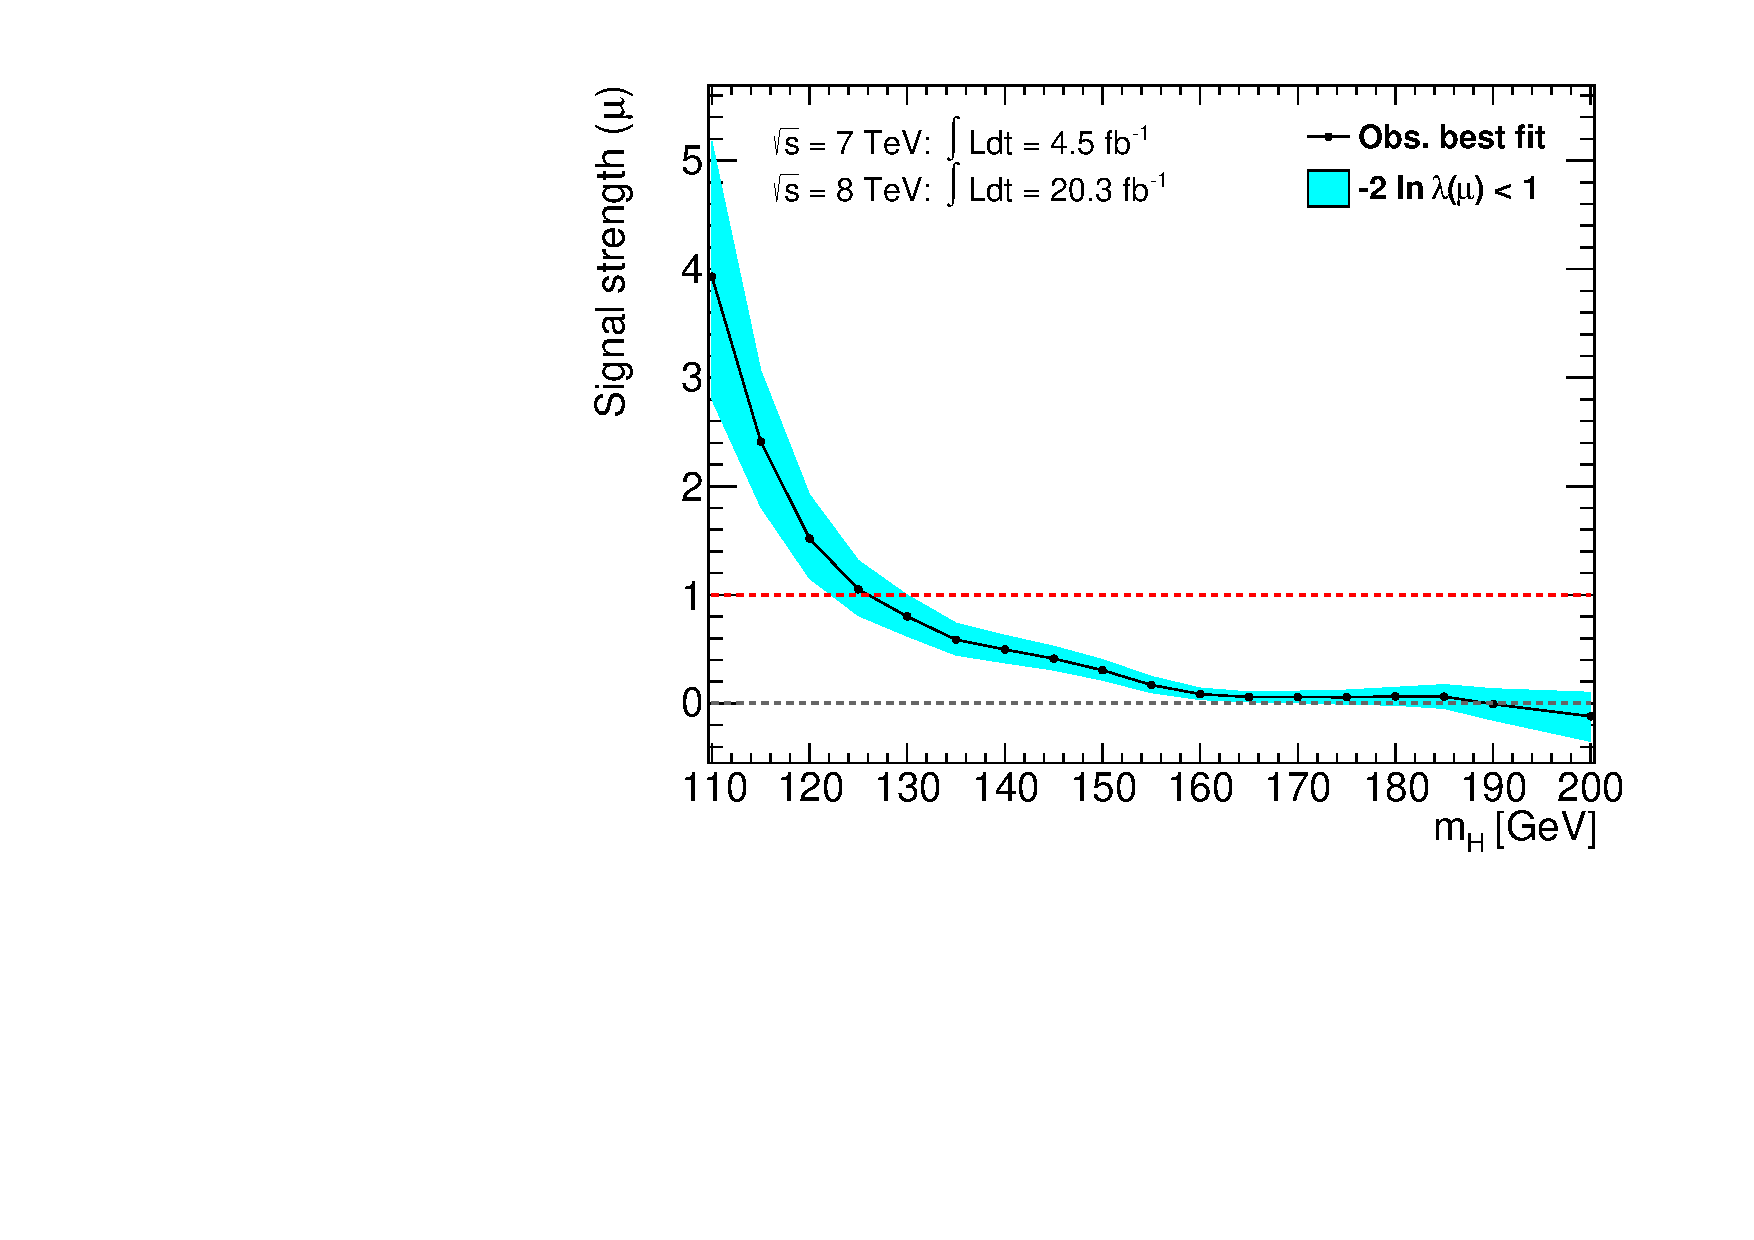
\includegraphics[width=\textwidth,clip=true,trim=0.6cm 0.8cm 1.0cm 0.4cm]{custom_images/limits/mu_ggf_only}
		\caption{Measurement of $\mu$}
		\label{fig:ggf_results:mu}
	\end{subfigure}
	\caption{Results of the ggF analysis. (a) The observed (solid) 95\% CL upper 
	limit on the signal strength $\mu$ as a function of the mass under test \mH, and the 
	expectation (dashed) under the background-only hypothesis. (b) The observed (solid) 
	$p_0$ as a function of \mH and the expectation (dashed) under the signal-plus-background 
	hypothesis with $\mu = 1$ and a hypothesised mass equal to that under test.	(c) The 
	best-fit signal strength $\hat{\mu}$ (solid) as a function of \mH, with the 68\% CL 
	interval shown (blue band).}
\end{figure}

The observed and expected (under a background-only hypothesis) 95\% CL upper limit on $\mu$ 
is shown as a function of the mass under test \mH in \Figure~\ref{fig:ggf_results:CLs}. The 
mass range where this limit is below unity is excluded at the 95\% CL, when considering an 
SM Higgs boson ($\mu = 1$). In the absence of a Higgs boson, the expected excluded region is 
\unit{116}{\GeV} to \unit{200}{\GeV}.\footnote{
	This analysis is optimised to search for a low-mass Higgs boson and therefore the region 
	\unit{$\mH > 200$}{\GeV} is not considered. A dedicated high-mass search for \HWW is 
	described in \Reference~\cite{HWW-highmass}.
}
However, the observed excluded region is \unit{132}{\GeV} to \unit{200}{\GeV}.
The fact that the observed exclusion is weaker than expected indicates an excess of 
events consistent with a Higgs boson. Since the mass resolution of the \HWW analysis is 
poor, the impact upon the exclusion is broad in \mH.

To quantify the significance of the excess of events, \Figure~\ref{fig:ggf_results:p0} shows 
the observed $p_0$ as a function of \mH. The maximum observed significance is $4.8\sigma$, 
which occurs when testing \unit{$\mH = 130$}{\GeV}, though the poor mass resolution leads to 
a relatively broad $p_0$ curve. This is very strong evidence for the existence of the Higgs 
boson, though does not pass the $5\sigma$ criterion for ``discovery''.

The best-fit signal strength $\hat{\mu}$ is shown as a function of the \mH under test in 
\Figure~\ref{fig:ggf_results:mu}. A range of Higgs boson masses are consistent with the 
assumption that the Higgs boson behaves as predicted by the SM (\ie $\mu = 1$). The data 
are also consistent with a lower mass Higgs boson with $\mu > 1$ or a higher mass Higgs 
boson with $\mu < 1$. 



\subsection{Combination with VBF analysis}
\label{sec:results:combined_limits}

The ggF analysis described in this thesis is combined with a multivariate VBF analysis, 
which selects events featuring two high-\pt jets separated by a large rapidity gap devoid of 
hadronic activity. This analysis features a higher signal-to-background ratio than the ggF 
analysis, but has a smaller expected number of events. It was briefly introduced in 
\Section~\ref{sec:selection:2j}, because the \twojet bin of the ggF analysis vetoes events 
selected by the VBF analysis in order to maintain orthogonality. The VBF analysis will be 
fully described in the upcoming paper \cite{HWW-RunI}.

The 95\% CL upper limit on $\mu$ is shown as a function of \mH in 
\Figure~\ref{fig:comb_results:CLs}. The expected (in the absence of a Higgs boson) excluded 
region is \unit{114}{\GeV} to \unit{200}{\GeV}, exhibiting only a small improvement upon the 
limit from the ggF analysis. The observed excluded region remains as \unit{132}{\GeV} to 
\unit{200}{\GeV}.

\begin{figure}[p]
	\begin{subfigure}[b]{0.495\textwidth}
		\centering
		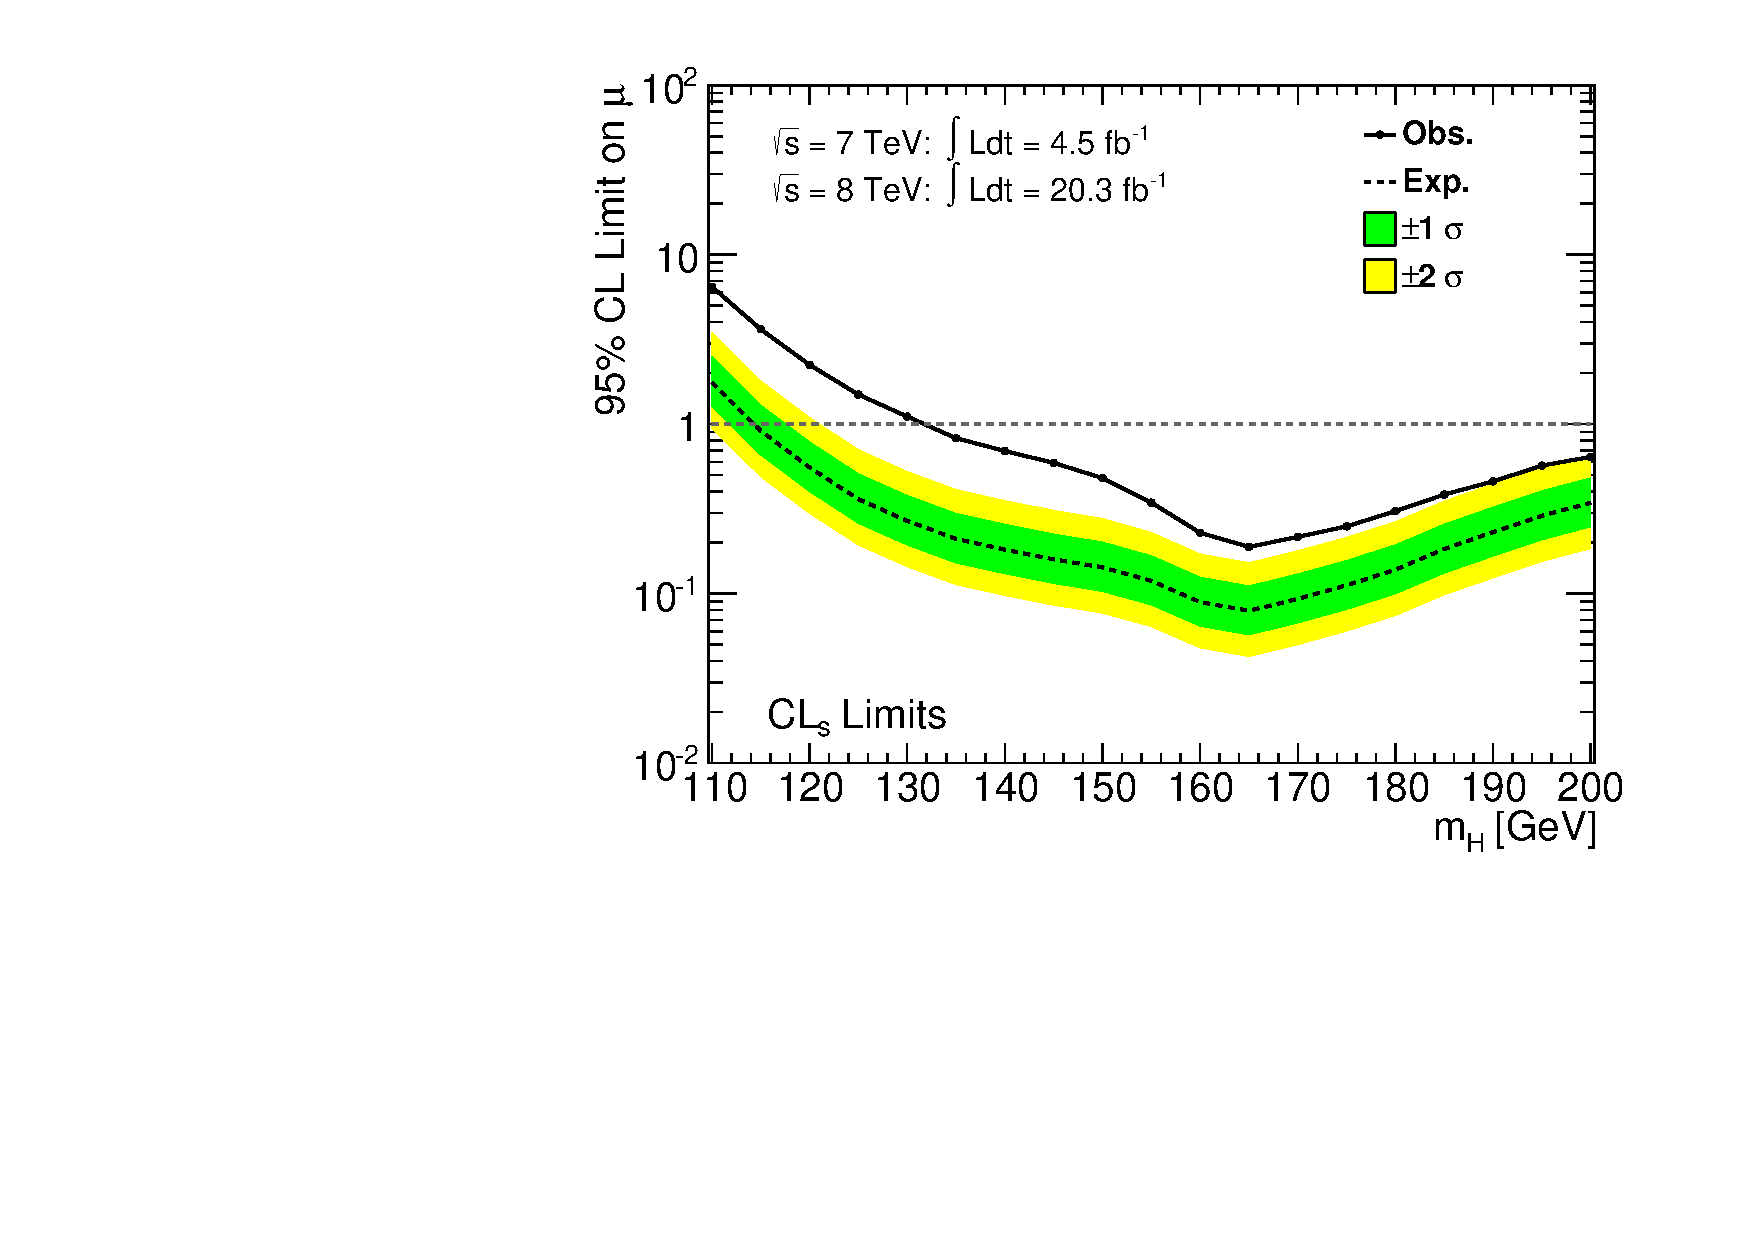
\includegraphics[width=\textwidth,clip=true,trim=0.6cm 0.8cm 1.0cm 0.4cm]{custom_images/limits/cls_combined}
		\caption{Exclusion}
		\label{fig:comb_results:CLs}
	\end{subfigure}
	\hfill
	\begin{subfigure}[b]{0.495\textwidth}
		\centering
		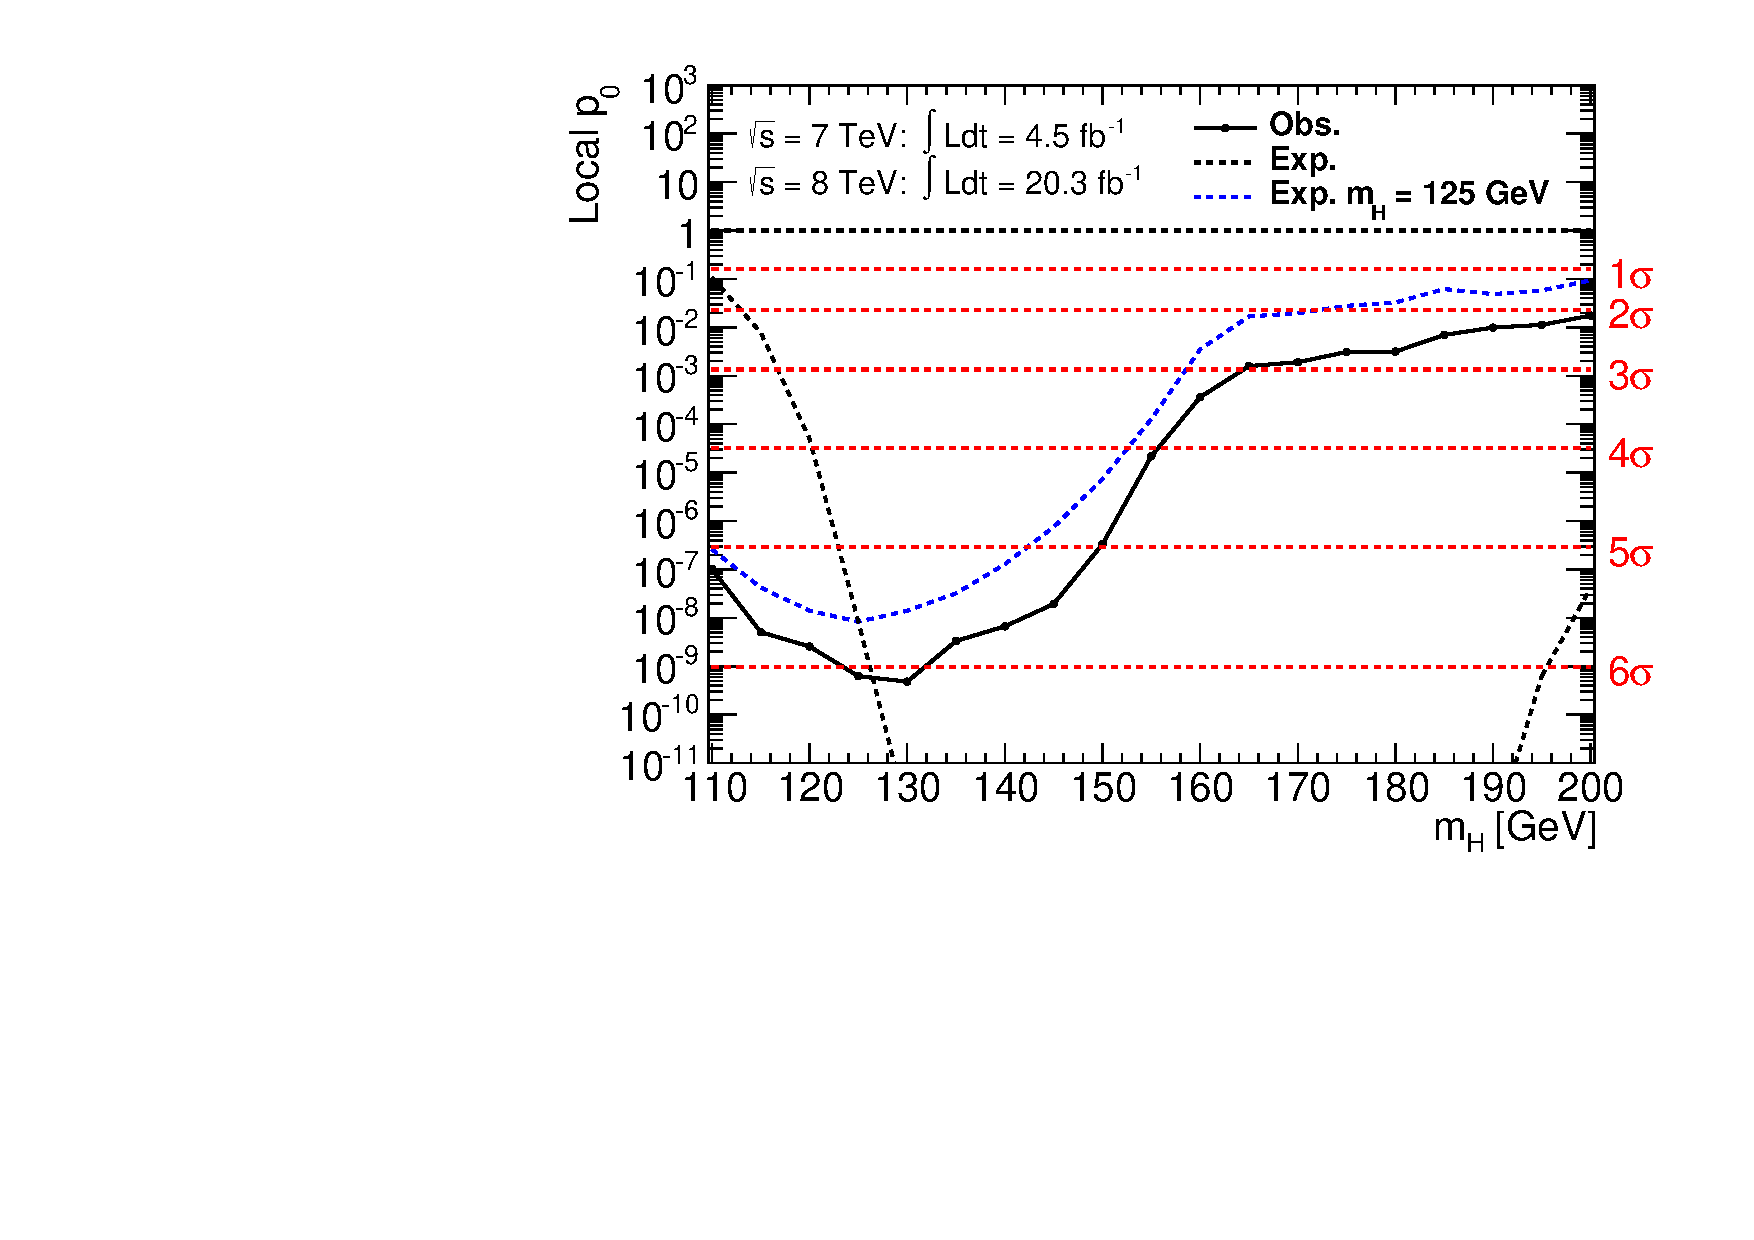
\includegraphics[width=\textwidth,clip=true,trim=0.6cm 0.8cm 1.0cm 0.4cm]{custom_images/limits/p0_combined}
		\caption{Discovery}
		\label{fig:comb_results:p0}
	\end{subfigure}
	\\[12pt]
	\begin{subfigure}[b]{0.495\textwidth}
		\centering
		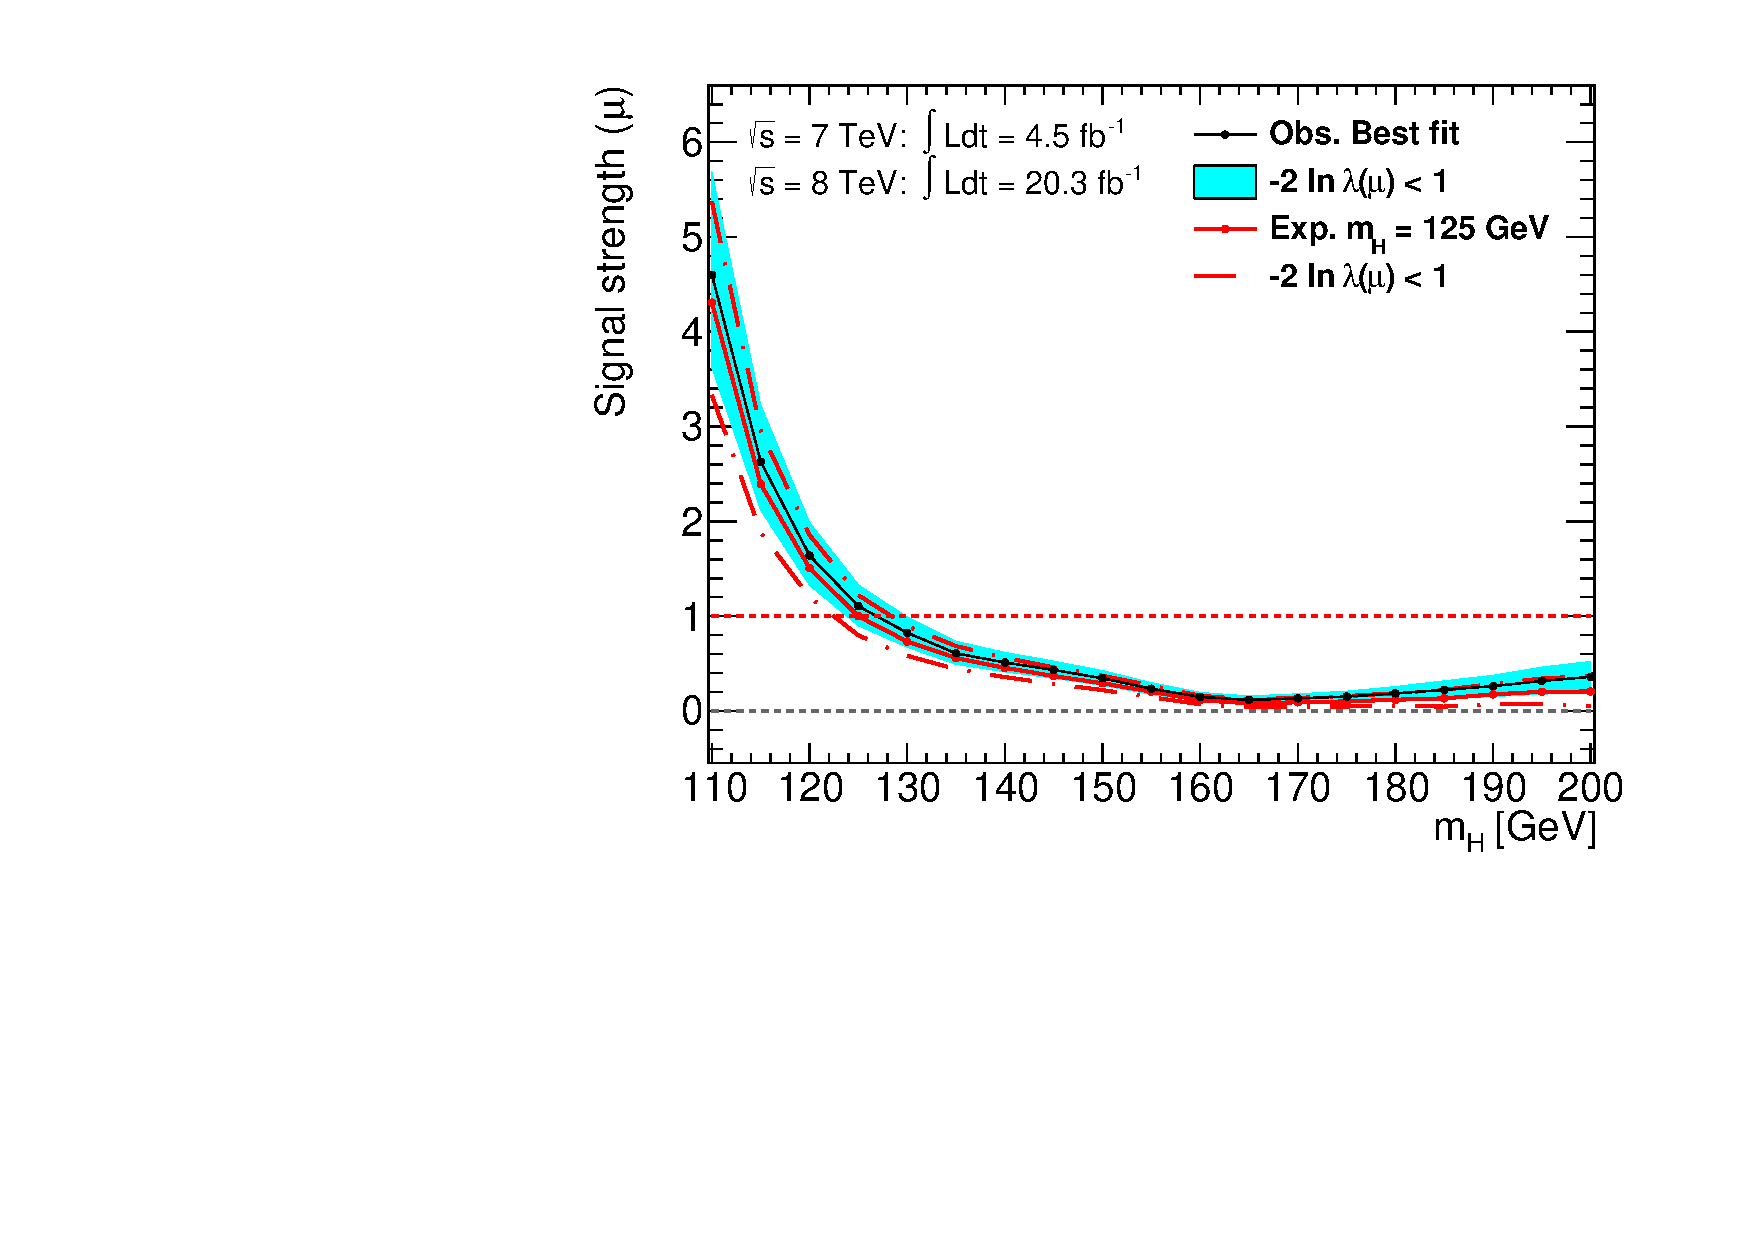
\includegraphics[width=\textwidth,clip=true,trim=0.6cm 0.8cm 1.0cm 0.4cm]{custom_images/limits/mu_combined}
		\caption{Measurement of $\mu$}
		\label{fig:comb_results:mu}
	\end{subfigure}
	\hfill
	\begin{subfigure}[b]{0.495\textwidth}
		\centering
		%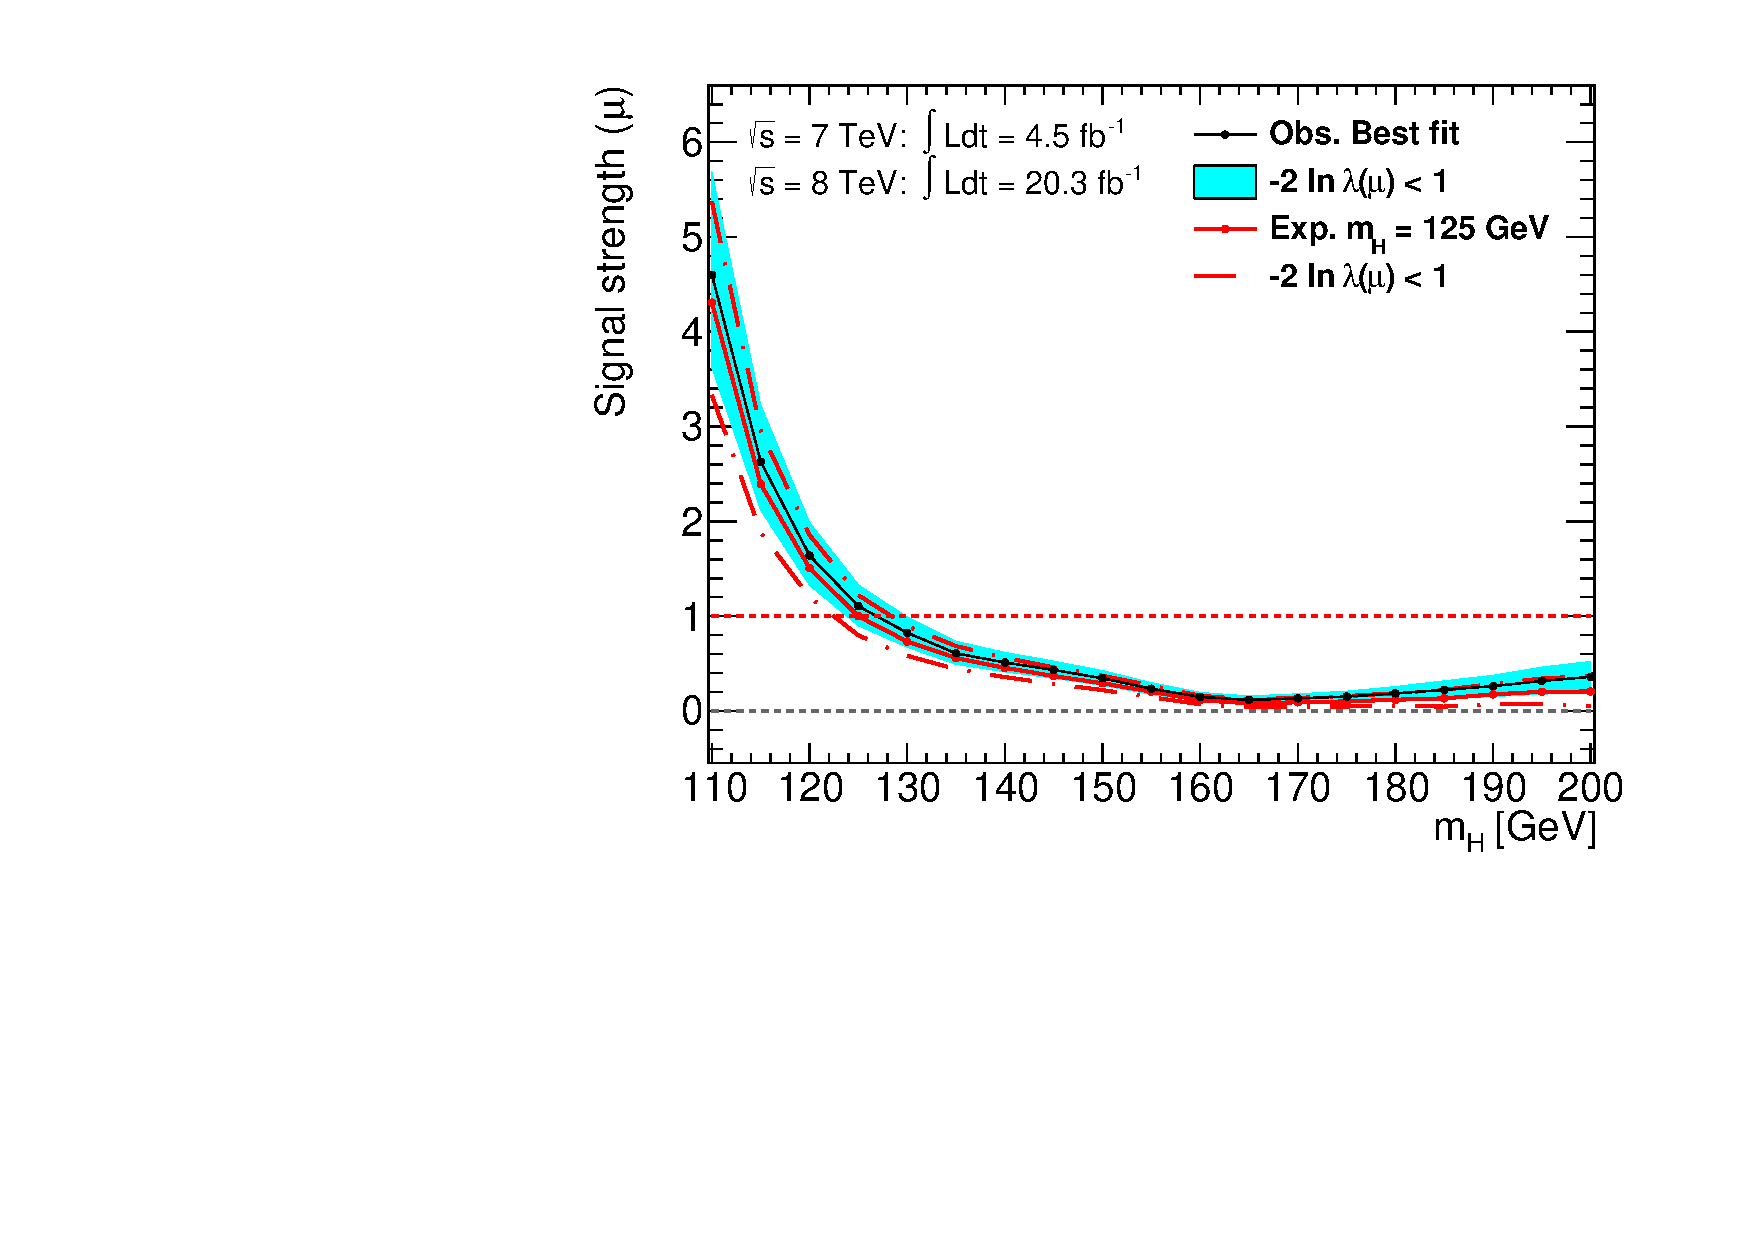
\includegraphics[width=\textwidth,clip=true,trim=0.6cm 0.8cm 1.0cm 0.4cm]{custom_images/limits/mu_combined}
		\caption{Measurement of $\parenths{\mu, \mH}$}
		\label{fig:comb_results:mu_mH}
	\end{subfigure}
	\caption{Results of the combined ggF+VBF analysis. (a) The observed (solid) 95\% CL 
	upper limit on the signal strength $\mu$ as a function of the mass under test \mH, and 
	the expectation (dashed) under the background-only hypothesis. (b) The observed (solid) 
	$p_0$ as a function of \mH and the expectation (black dashed) under the 
	signal-plus-background hypothesis with $\mu = 1$ and a hypothesised mass equal to that 
	under test.	The expectation (blue dashed) for a hypothesised mass 
	\unit{$\mH = 125$}{\GeV} is also shown. (c) The best-fit signal strength $\hat{\mu}$ 
	(solid) as a function of \mH, with the 68\% CL interval shown (blue band). The 
	expectation (red) for a hypothesised mass \unit{$\mH = 125$}{\GeV} is also shown. 
	(d) The best-fit signal strength $\hat{\mu}$ and mass $\hat{m}_{\PHiggs}$ (marker), with 
	the 68\% CL and 95\% CL intervals shown.}
\end{figure}

The observed $p_0$ is shown in \Figure~\ref{fig:comb_results:p0} as a function of the mass 
under test \mH.  The maximum observed significance is $6.1\sigma$, occurring when testing 
\unit{$\mH = 130$}{\GeV}. This constitutes a discovery of the Higgs boson, made by searching 
for the ggF and VBF production modes and the \WW decay channel.

The best-fit signal strength $\hat{\mu}$ is shown as a function of the \mH under test in 
\Figure~\ref{fig:comb_results:mu}. By including \mH as a parameter of interest in the fit, 
it is possible to test which $\parenths{\mu, \mH}$ pair are most favoured by the data. This 
is presented in \Figure~\ref{fig:comb_results:mu_mH}, together with the 68\% CL and 95\% CL 
contours. This clearly demonstrates that the analysis is more sensitive to $\mu$ than to \mH.

These results exhibit more than $5\sigma$ significance for \HWWlvlv, and consequently for 
the existence of the Higgs boson itself. LHC searches for 
\HepProcess{\PHiggs \HepTo \Pphoton\Pphoton} and \HepProcess{\PHiggs \HepTo \PZ\PZ} have 
found consistent evidence, which is summarised in \Section~\ref{sec:searches}. These two 
channels yield much better mass sensitivity, and observe \unit{$\mH \approx 125$}{\GeV}. 
For this reason, the expected $p_0$ and $\hat{\mu}$ under the assumption of a SM Higgs boson 
with \unit{$\mH = 125$}{\GeV} are also included in Figures~\ref{fig:comb_results:p0} and 
\ref{fig:comb_results:mu} respectively. It can be seen that the observed $p_0$ is smaller 
than expected (\ie the significance of the incompatibility with the null hypothesis is 
greater), though the shape remains consistent. This feature of the data is also expressed by 
the best-fit $\hat{\mu}$ being greater than unity ($\hat{\mu} = 1.11 \pm 0.22$) at 
\unit{$\mH = 125$}{\GeV}. The excess of events is further characterised in 
\Figure~\ref{fig:comb_results:p0_mu_breakdown}.

\begin{figure}[p]
	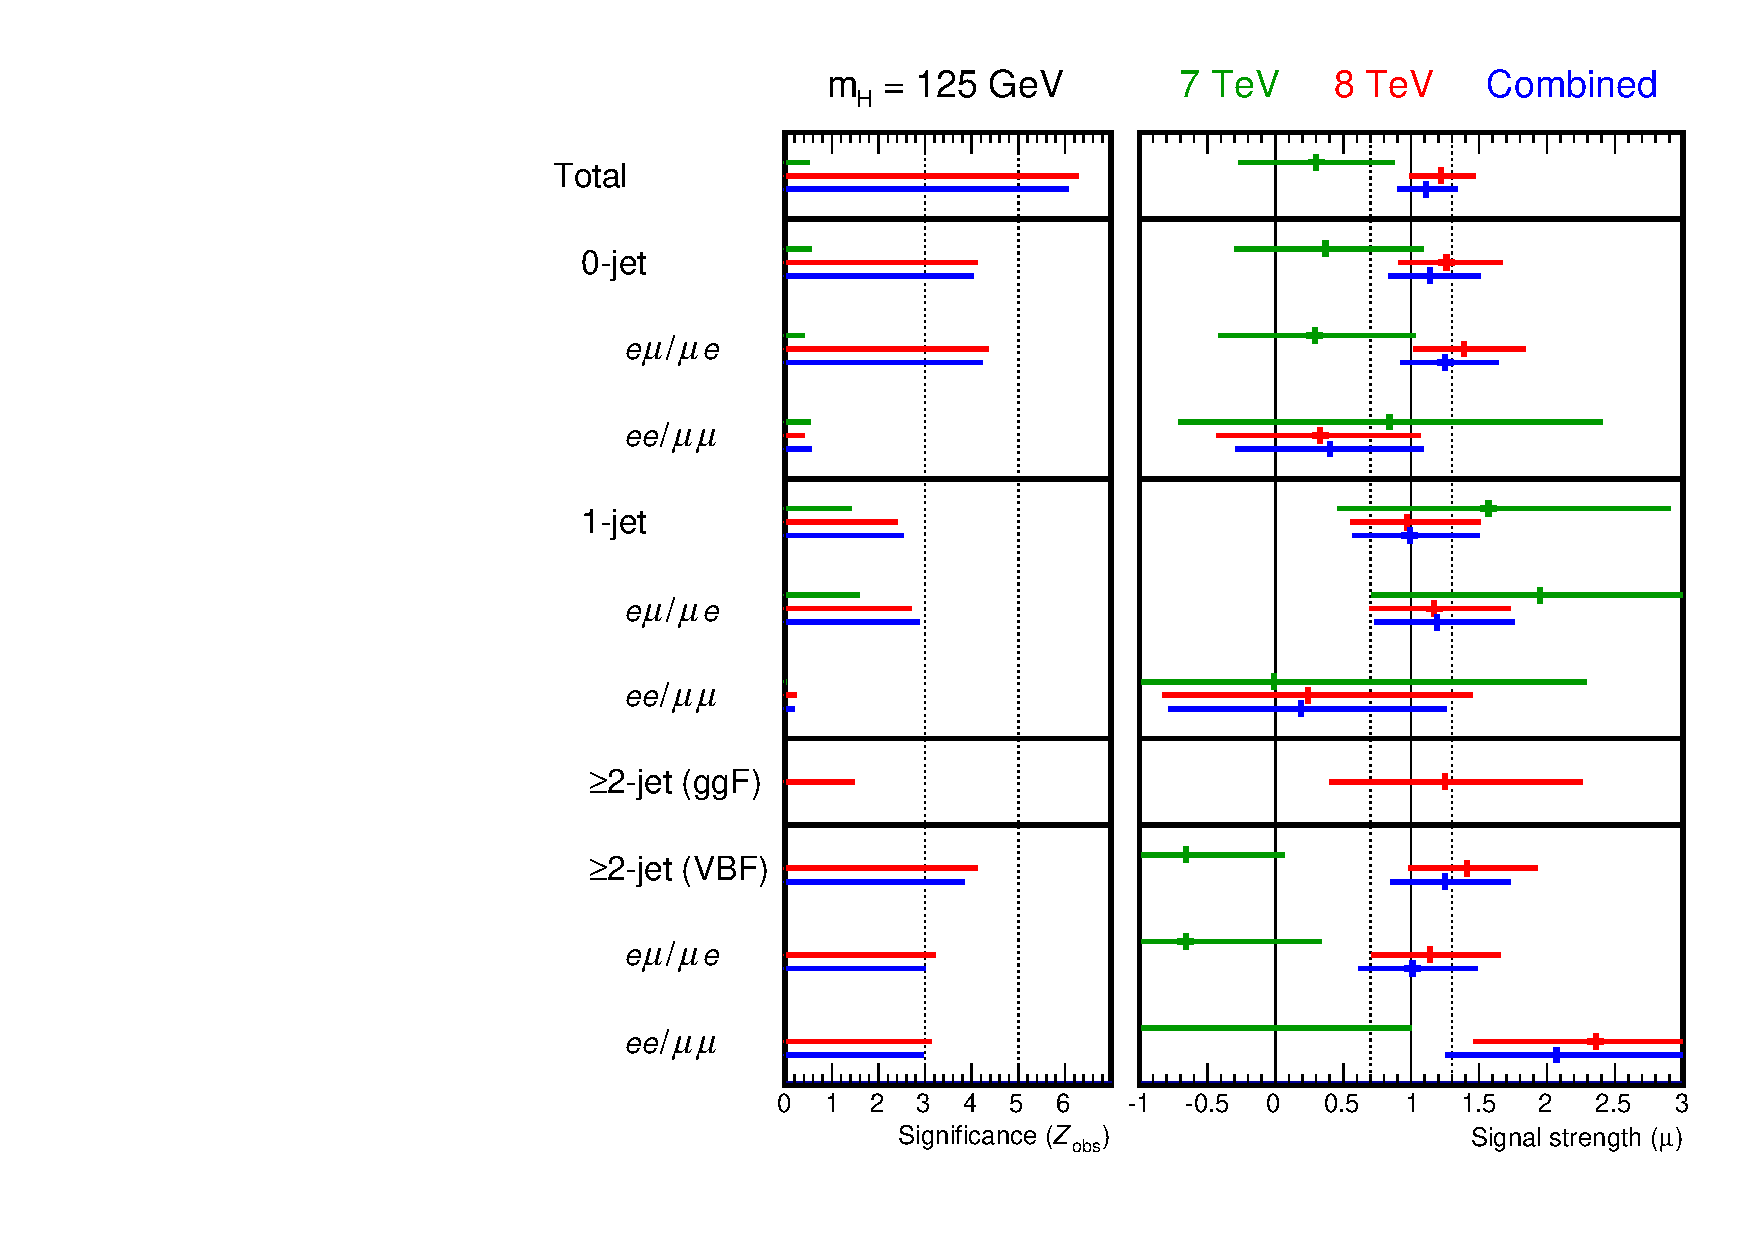
\includegraphics[width=\hugefigwidth]{custom_images/limits/z_and_mu}
	\caption{The observed significance in units of Gaussian standard deviations, $Z$, and 
	the measured signal strength, $\hat{\mu}$, when testing \unit{$\mH = 125$}{\GeV}. The 
	contribution of each signal region is shown. The fit results using the 
	\unit{$\sqrt{s} = 7$}{\TeV} dataset (green), the \unit{$\sqrt{s} = 8$}{\TeV} dataset 
	(red), and their combination (blue) are also separated.}
	\label{fig:comb_results:p0_mu_breakdown}
\end{figure}

It is possible to assign the ggF and VBF production modes independent signal strength 
parameters, with $\mu_{\text{ggF}}$ constrained by the ggF analysis and 
$\mu_{\text{VBF}}$ constrained by the VBF analysis. This is interesting because they 
are dominated by different types of Higgs coupling, and the loop in the ggF process can be 
sensitive to undiscovered massive particles. When doing this, the \VH production mode is 
assigned the same signal strength as VBF because they are both dominated by bosonic 
couplings. The resulting limits upon $\parenths{\mu_{\text{ggF}}, \mu_{\text{VBF}}}$ are 
shown in \Figure~\ref{fig:comb_results:muvbf_vs_muggf}. It can be seen that both ggF and VBF 
are in excellent agreement with the SM, though VBF is observed to be produced more often 
than expected.

\begin{figure}[t]
	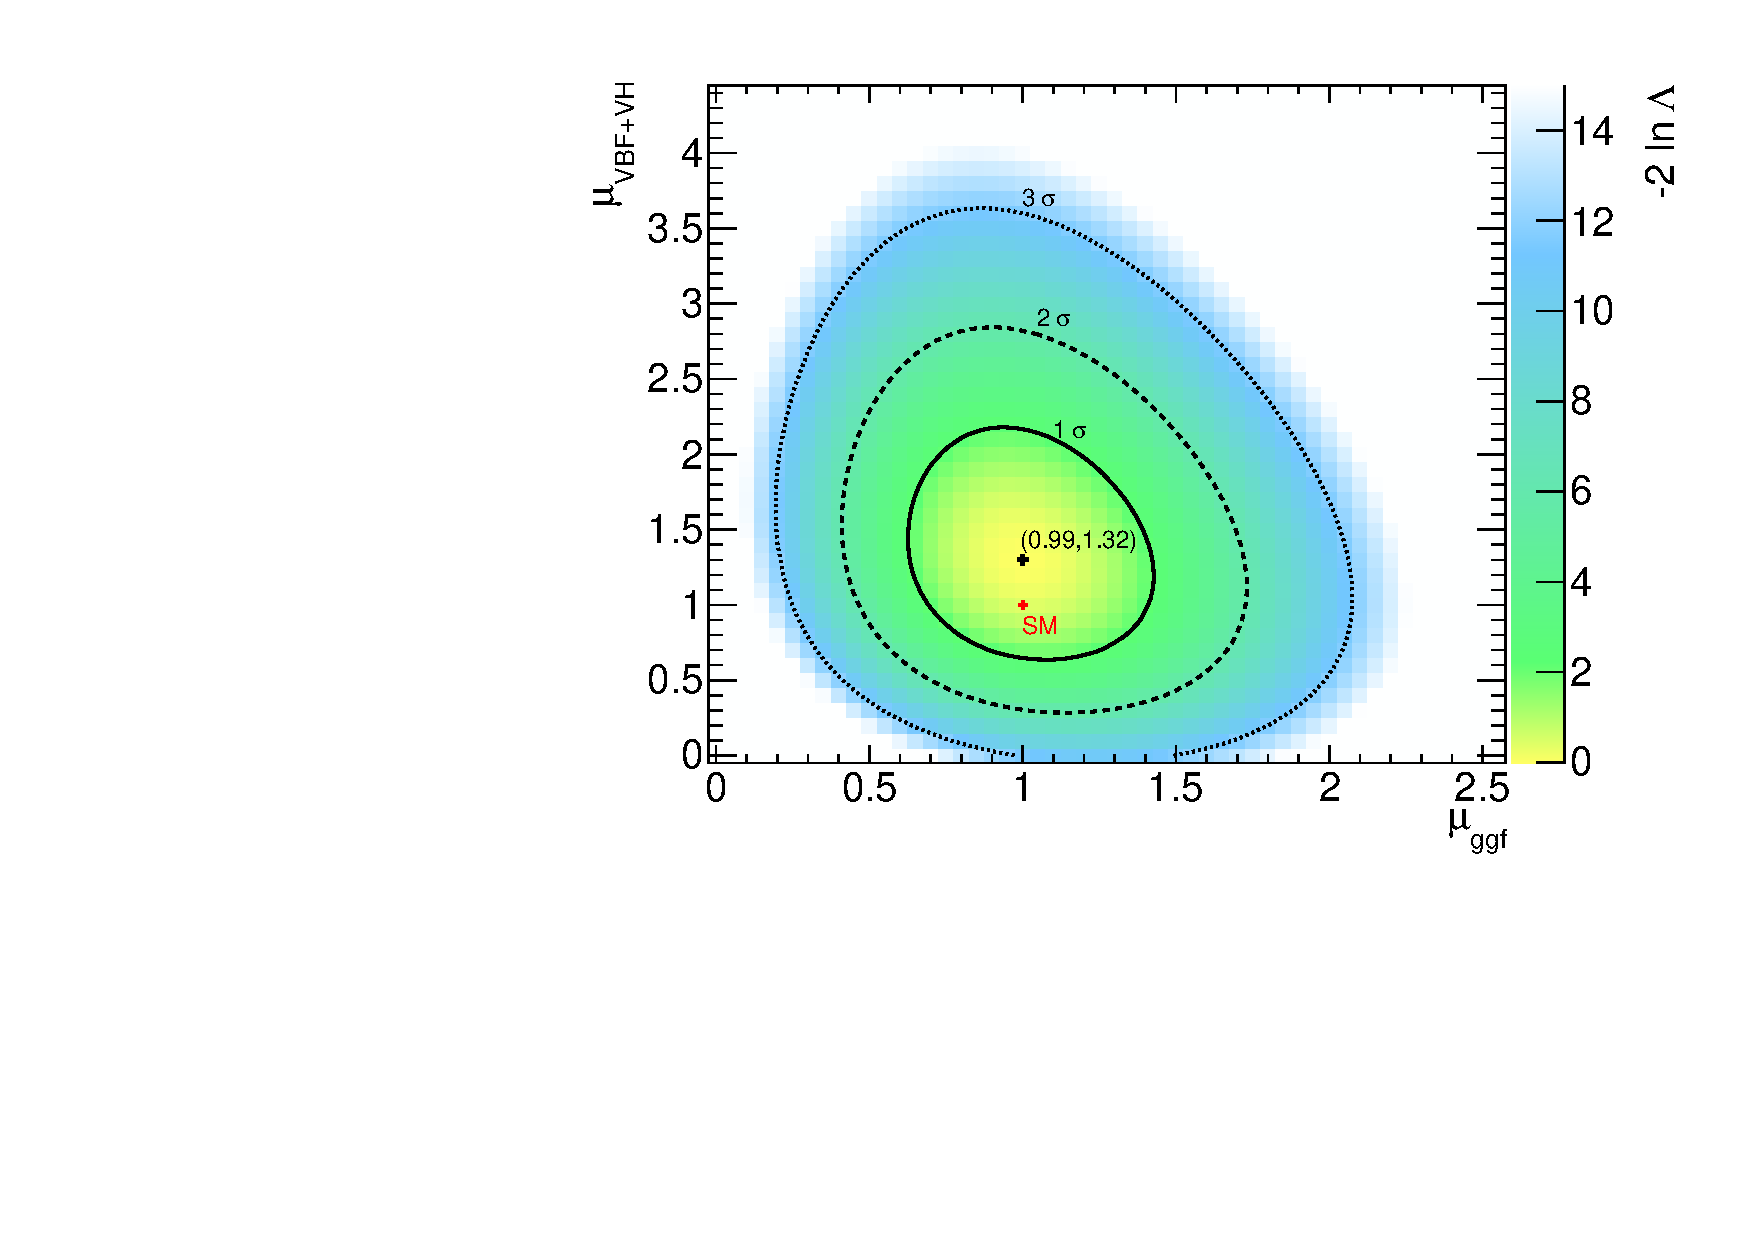
\includegraphics[width=\mediumfigwidth]{custom_images/limits/muvbf_vs_muggf}
	\caption{Likelihood contours for $\mu_{\text{ggF}}$ and $\mu_{\text{VBF+VH}}$, when 
	testing \unit{$\mH = 125$}{\GeV}. The markers show the best-fit values observed 
	(black) and expected under an \unit{$\mH = 125$}{\GeV} hypothesis (red).}
	\label{fig:comb_results:muvbf_vs_muggf}
\end{figure}

\Table~\ref{tab:comb_results:mu_uncertainties} shows a breakdown of the uncertainties in 
$\hat{\mu}$. It can be seen that $\hat{\mu}_{\text{VBF}}$ is dominated by statistical 
uncertainties, whereas $\hat{\mu}_{\text{ggF}}$ is almost equally limited by statistical 
and systematic uncertainties. It should be noted that theoretical uncertainties 
(particularly in signal modelling) are the largest source of systematic uncertainty, 
highlighting the importance of the ggF and \WW studies in Chapters~\ref{chap:signal} and 
\ref{chap:ww} respectively.

\begin{table}[p]
	\begin{tabularx}{0.8\textwidth}{l@{\hskip 0.3in}*{3}{Z}}
		\toprule
		& \multicolumn{3}{c}{Relative uncertainty $\Delta\mu/\mu$ (\%)} \\
		& ggF & VBF & Combined \\
		\midrule
		Statistical                          & 20 & 33 & 16 \\
		\cmidrule{2-4}
		\quad Signal regions                 & 14 & 29 & 12 \\
		\quad Control regions                & 12 & 15 &  9 \\
		\quad Signal contamination           &  3 &  7 &  0 \\
		\quad Finite MC size                 &  6 &  4 &  4 \\
		\cmidrule{1-4}
		Systematic                           & 18 & 21 & 13 \\
		\cmidrule{2-4}
		\quad Experimental                   & 10 & 13 &  8 \\
		\cmidrule{2-4}
		\quad\quad Leptons and triggers      &  5 &  2 &  4 \\
		\quad\quad Jets and \Pbottom-tagging &  3 & 10 &  2 \\
		\quad\quad \met modelling            &  2 &  4 &  2 \\
		\quad\quad Fake factor               &  8 &  2 &  5 \\
		\quad\quad Other                     &  4 &  5 &  3 \\
		\cmidrule{2-4}
		\quad Theoretical                    & 15 & 16 & 11 \\
		\cmidrule{2-4}
		\quad\quad Signal modelling          & 11 & 14 &  9 \\
		\quad\quad Background modelling      &  9 &  8 &  7 \\
		\cmidrule{2-4}
		\quad Luminosity                     &  3 &  4 &  3 \\
		\bottomrule
		\toprule
		Total                                & 26 & 39 & 20 \\
		\bottomrule
	\end{tabularx}
	\caption{A breakdown of the relative uncertainty upon the fitted signal strengths 
	$\hat{\mu}_{\text{ggF}}$ and $\hat{\mu}_{\text{VBF}}$, and in the combined signal 
	strength $\hat{\mu}$. ``Signal contamination'' refers to how the finite number of 
	events in the signal region of the VBF analysis introduces a statistical uncertainty in 
	the expected number of VBF events in the signal region of the ggF analysis, and vice 
	versa.}
	\label{tab:comb_results:mu_uncertainties}
\end{table}


\clearpage
\subsection{Cross section measurements}
\label{sec:results:xs}

Following the method described in \Section~\ref{sec:ggF:acc}, fiducial ggF cross sections 
are extracted for fiducial regions defined for the 0-jet and 1-jet bins of the \emch{}+\mech 
channel. These are only extracted at \unit{$\sqrt{s} = 8$}{\TeV}. This is done using
\begin{equation}
	\sigma^{\text{fid}}_{\text{ggF}}
	&= \frac{N_{\text{obs}} - N_{\text{bkg}}}{C_{\text{ggF}} \cdot L} \\
	&= \hat{\mu}_{\text{ggF}} \cdot \sigma_{\text{ggF}}^{\text{SM}} \cdot \text{BR}^{\text{SM}} \cdot A_{\text{ggF}}
\end{equation}
where $L$ is the luminosity, $C_{\text{ggF}}$ is the ratio of the expected number of ggF 
events passing the detector-level selection to those passing the fiducial selection, and 
$A_{\text{ggF}}$ is the ratio of the expected number of ggF events passing the fiducial 
selection to the total expected number of ggF events. Here, $\hat{\mu}$ is determined by a 
dedicated fit in which the nuisance parameters associated with theoretical uncertainties in 
the total ggF cross section, the BR and the ggF acceptance are fixed, such that their effect 
upon $\Delta\mu$ is removed. The VBF and \VH processes are set to their SM expectations 
(\ie $\mu_{\text{VBF}} = 1$). The measured fiducial cross sections for 
\unit{$\mH = 125$}{\GeV} are displayed in \Table~\ref{tab:results:xs_fiducial}. The measured 
values are higher than predicted, which is consistent with 
\Figure~\ref{fig:comb_results:p0_mu_breakdown}.

\begin{table}[t]
	\begin{tabular}{c@{\hskip 0.3in}r@{$\,\pm\,$}r@{$\,\pm\,$}r@{\hskip 0.3in}r@{$\,\pm\,$}l}
		\toprule
		Fiducial & \multicolumn{5}{c}{$\sigma^{\text{fid}}$ (fb)} \\
		region & \multicolumn{3}{@{}c@{\hskip 0.3in}}{Measured} & \multicolumn{2}{@{}c}{Predicted} \\
		\midrule
		0-jet \emch{}+\mech & 28.1 & 5.5 & 4.1 & 19.9 & 3.3 \\
		1-jet \emch{}+\mech &  8.4 & 3.1 & 1.9 &  7.3 & 1.8 \\
		\bottomrule
	\end{tabular}
	\caption{Measured fiducial ggF cross sections at \unit{$\sqrt{s} = 8$}{\TeV}, assuming 
	\unit{$\mH = 125$}{\GeV}. Theoretical predictions are shown for comparison. The 
	uncertainties in measured quantities are statistical and systematic, respectively.}
	\label{tab:results:xs_fiducial}
\end{table}

The product of the total cross section and the \HWW branching ratio is extracted for ggF (at 
\unit{$\sqrt{s} = 7$}{\TeV} and \unit{8}{\TeV}) and VBF (at \unit{$\sqrt{s} = 8$}{\TeV}) 
using
\begin{equation}
	\sigma_i \cdot \text{BR} 
	&= \frac{N_{\text{obs}} - N_{\text{bkg}}}{C_i \cdot A_i \cdot L} \\
	&= \hat{\mu}_i \cdot \sigma_i^{\text{SM}} \cdot \text{BR}^{\text{SM}}
\end{equation}
where $i = \text{ggF, VBF}$. The $\hat{\mu}_i$ are determined by a dedicated fit in which 
the nuisance parameters associated with theoretical uncertainties in the total cross 
sections and branching ratio are fixed, such that their effect is removed. When 
$\hat{\mu}_{\text{ggF}}$ is measured $\mu_{\text{VBF}}$ is profiled, and vice versa. The 
measured cross sections for \unit{$\mH = 125$}{\GeV} are displayed in 
\Table~\ref{tab:results:xs_total} and show good agreement with the theoretical predictions.

\begin{table}[t]
	\begin{tabular}{cc@{\hskip 0.3in}r@{$\,\pm\,$}r@{$\,\pm\,$}r@{\hskip 0.3in}r@{$\,\pm\,$}r}
		\toprule
		\multirow{2}{*}{Process} & \multirow{2}{*}{$\sqrt{s}$} & \multicolumn{5}{c}{$\sigma \cdot \text{BR}$ (pb)} \\
		&  & \multicolumn{3}{@{}c@{\hskip 0.3in}}{Measured} & \multicolumn{2}{@{}c}{Predicted} \\
		\midrule
		ggF & \unit{7}{\TeV} & 1.7\phantom{0} & 1.8\phantom{0} & 1.2\phantom{0} & 3.3\phantom{39} & 0.4\phantom{00} \\
		ggF & \unit{8}{\TeV} & 4.7\phantom{0} & 0.8\phantom{0} & 0.8\phantom{0} & 4.1\phantom{39} & 0.5\phantom{00} \\
		VBF & \unit{8}{\TeV} & 0.53 & 0.16 & 0.10 & 0.339 & 0.017 \\
		\bottomrule
	\end{tabular}
	\caption{Measured ggF and VBF total cross sections multiplied by the \HWW branching 
	ratio, assuming \unit{$\mH = 125$}{\GeV}. Theoretical predictions are shown for 
	comparison. The uncertainties in measured quantities are statistical and systematic, 
	respectively.}
	\label{tab:results:xs_total}
\end{table}
